\documentclass[11pt]{article}

\usepackage[a4paper, margin=2cm,headsep=6pt]{geometry}
\usepackage{lineno}
\usepackage[utf8]{inputenc}
\usepackage[english]{babel}
\usepackage{graphicx}
\usepackage{amsmath}
\usepackage{multirow}
\usepackage{caption}
\usepackage{array}
\usepackage{float}
\usepackage{csvsimple}
\usepackage{rotating}
\usepackage{lscape}
\usepackage{adjustbox}
\newcolumntype{P}[1]{>{\centering\arraybackslash}p{#1}}
\newcommand{\soptitle}{Detecting differences between strains of Cryptococcus neoformans through a new tool in detecting ploidy}
\usepackage{fancyhdr}
\pagestyle{fancy}
\linespread{1.25}
\fancyhead[R]{CID 01383312}
\fancyhead[L]{Oliver Tarrant}
\usepackage{csquotes}
\usepackage[backend=bibtex,style=authoryear]{biblatex}

\bibliography{Project.bib}
\begin{document}
\begin{titlepage}
\begin{center}
\hrule
\vspace{2pt}
\hrule
\vspace{2cm}
\LARGE {\bf \underline{CMEE Project}}\\
\vspace{2cm}
\huge{\bf \soptitle}\\
\vspace{4cm}
\LARGE {\bf Oliver Tarrant}\\
\large{Imperial College London, Department of Biological Sciences}\\
\large{MRes Computational Methods in Ecology and Evolution}\\
\vfill
\large{Word count: }\\
\huge {\bf Supervised by Dr. Matteo Fumagalli}\\
\large {m.fumagalli@imperial.ac.uk} 
\end{center}
\hrule
\vspace{2pt}
\hrule
\end{titlepage}
\linenumbers


\section{Abstract}

\section{Introduction}
\paragraph{}Cryptococcus neoformans is an opportunistic fungi that is responsible for up to 30\% of AIDs related deaths through infections of Crytococcus Meningitis (CM) \autocite{Vanhove2016}. Part of the reason for its success as a pathogen is its ability to evolve quickly within its hosts \autocite{Rhodes2017}. This micro-evolution seems to occur through multiple pathways with one of the most important being through the production of copy number variation (CNV). CNV is the presence of extra or missing copies of genes within a genome \autocite{Joao2015}. The occurrence of CNV of an entire chromosome is referred to as aneuploidy or chromosomal copy number variation (CCNV). In C.neoformans, CCNV of certain areas of the genome increase the concentration of drug resistant genes promoting more virulent stands of CM \autocite{Rhodes2017}.
\paragraph{}It is believed that CNV arise predominantly through misalignments during meiotic recombination and methods such as breakage-fusion-bridge cycles or non-homologous end joining \autocite{Hastings2010}. 
\paragraph{}A recent paper on C.neoformans \autocite{Rhodes2017} focused on 17 HIV infected individuals from sub-Saharan Africa. Each individual had contracted CM and after initial treatment had been reinfected. The study concluded that 15 of the individuals had suffered a relapse of their original infection whilst for the remaining two, one had been initially infected by a mixture of strains whilst the infection in the other patient had developed a hyper-mutator state and thus formed a new strand. Those infections that caused relapses within the patients showed high levels of CCNV as a pathway for within host evolution to form a drug resistant isolate. 
\paragraph{}Research within this paper was restricted by the uncertainty surrounding the genotypes of the isolates. In particular .....INCLUDE RESTRICTIONS.... 
\paragraph{}The aim of this study was predominately to utilise the new techniques developed to accurately detect the cases of CCNV within the dataset of c.neofromans isolates. With the resulting information, the gentic diversity of the isolates was studied providing a more realistic estimation from those derived with the original assumptions. By using the actual ploidy levels present it has also been possible to investigate the effect of including this extra level of complexity into the phylogenetic analysis of the isolates. After improving the assumptions on the phylogenetic clustering and genetic diversity more power was available to study the genes under selection within the isolates thus providing a better idea at the affects of microeveolution caused by drug pressures for the C.neoformans fungi. All together these tests were performed to quantify and qualify the differences between the separate lineages of the C.neoformans fungus and to understand the role of CCNV within these differences.  





%Introduction. A good introduction should leave the reader with a clear idea of the problem to be tackled and looking forward to the more detailed sections to follow. It should include a section on the general way the problem has been approached. An essential concluding part of the introduction is to clearly define the aims of the research project and any hypotheses tested. Also, think about: o What is this paper about? (i.e., the broad area, big picture) Why is that interesting? o Given it’s so interesting, why don’t we know the answer? o So, what is this about, more specifically? What are hypothesised to be the important things? Build from the most general and fundamental hypotheses to the most refined or tenuous ones. o How, roughly and briefly, will you go about testing these hypotheses? Why are you using this system? What approach will you use? o State clearly what your hypotheses are. These are not usually stated explicitly in a paper.

\section{Methods}
\subsection{Data wrangling}
\paragraph{}The data is first filtered for monomorphic sites. A monomorphic site (one where only one allele can be found) is not informative of the ploidy as it would be impossible to distinguish between the likelihoods of genotypes. Thus to remove excess noise, the data is filtered so that remaining bases all have a major allele frequency of less than 0.8. Thus the remaining data are the single nucleotide polymorphisms (SNPs). 
\paragraph{}To save on computational time the triallelic and tetrallelic sites are also filtered out. The proportions of the third and fourth most common allele at the site are calculated, if greater than 0.1 then the site is also removed. Thus genotype likelihoods are calculated for these sites assuming they are biallelic. Evidently the most likely genotype at a site was triallelic then it would imply the individual had a ploidy level $>2$ (and $>3$ if tetrallelic). Whilst being a limitation of this method, it is likely that the added information from including these sites would be outweighed by the extra computational time required.


%Current research uses a hidden markov chain model to determine detect the ploidy levels present in an organism's genome. The model takes into account the base quality and depth that a region was sequenced at when determining its ploidy. These inclusions help to counter sequencing errors and the corresponding uncertainty in genotype calling that occur with next generation sequencing (NGS) data. In particular the model re-evaluates the assumptions of diploidy and random mating which are commonly found throughout available software used to calculate genetic diversity. Performance of this model on simualted data demonstrates accurate estimations for trajectories of ploidy levels, even for data of depths as low as 2x.
\subsection{Genotype likelihoods}
\paragraph{}Denote by $O_{i,j}$, all the read information observed for individual $i$ at base position $j$. Thus $O_{i,j}$ consists of a list of two element components, the first of which is the nucleotide reads observed, denoted $o_{i,j}$, and the second are the corresponding phred quality scores denoted $q_{i,j}$. The phred quality scores can be converted into the probability that a base has been incorrectly called by using the relationship shown in equation \ref{phred}.

\begin{equation}\label{phred}
bP=10^{-Q/10}
\end{equation} 

The genotype likelihood at base position $j$ for an individual $i$ is the likelihood of observing genotype $G_{i,j}$ at that base. The log-likelihood of the data given each genotype can be observed by using a baysian approach taken from \autocite{Nielsen2011} as outlined below: 

\begin{equation}\label{geno_likes}
ln[P(O_{i,j}|G_{i,j},y_{i,j})]=\sum_{r=1}^{R}ln[\sum_{k=1}^{y_{i,j}}\frac{1}{y_{i,j} }P(o_{i,j,r}|g_{i,j,k},q_{i,j,r},y_{i,j})]
\end{equation} 

Where

\begin{equation}
P(o_{i,j,r}|g_{i,j,k},q_{i,j,r},y_{i,j})=
	\begin{cases} 
		1 - \epsilon_{i,j,r}, & \textit{if } o_{i,j,r} = g_{i,j,k} \\
    	\frac{\epsilon_{i,j,r}}{3} & \textit{otherwise}
	\end{cases}
\end{equation}

$R$ is the total number of reads and $y_{i,j}$ is the ploidy level for individual $i$ at base $j$. $g_{i,j,k}$ represents the k'th value of the genotype $G_{i,j}$.
\subsection{Ploidy likelihood}
\paragraph{}The overall likelihood that a sample has ploidy level $y_{i}$ can be calculated as shown in equation \ref{sam_like} by summing across the likelihoods of each genotype belonging to that ploidy at each base and then multiplying across all the bases.

\begin{equation}\label{sam_like}
ln[P(O_{i}|y_{i})]=\sum_{j=1}^{N}ln[\sum_{G_{i,j} \in S_{y_{i} }} P(O_{i,j}|G_{i,j},y_{i,j})P(G_{i,j}|y_{i,j})]
\end{equation}

Here $S_{y_{i} }$ is the set of genotypes that are possible for ploidy $y_{i}$, $N$ the number of all bases in the supercontig. The value of $P(G_{i,j}|y_{i,j})$ is approximated assuming that the alleles at each base are in Hardy-Weinberg equilibrium (HWE). A major and minor allele are assigned by calculating the genotype likelihoods of each allele being haploid from $O_{i,j}$ (see \ref{geno_likes}). The allele with greatest likelihood is then classed as the major allele at that base and the second most likely the minor allele. The allele frequencies are then estimated by weighting the read available by their quality score as follows:

\begin{equation*}
\bar{P}=P(\textit{Major allele at base j})=\frac{ \textit{Sum of phred scores for major alleles at base j} }{\textit{Sum of phred scores for major and minor alleles at base j} }
\end{equation*}
\begin{equation*}
\bar{Q}=P(\textit{Minor allele at base j})=\frac{\textit{Sum of phred scores for minor alleles at base j} }{\textit{Sum of phred scores for major and minor alleles at base j} } =1-\bar{P}
\end{equation*}

Thus we can apply HWE assumptions and calculate:

\begin{equation}
P(G_{i,j}=n_{1}\times\textit{major},n_{2}\times\textit{minor}|y_{i,j})=\binom{n_{1} + n_{2} }{n_{1} } \bar{P}^{n_1} \bar{Q}^{n_2} 
\end{equation}

To further increase the accuracy of this calculation, the co-efficient of inbreeding, $F$, has been included \autocite{Vieira2013}. $F$ is an estimate for the proportion of the population that is inbred \autocite{Howard2017}. Thus now the frequency of $G_{i,j}$ can be expressed as a sum of terms representing the probability that the individual is not inbred with genotype $G_{i,j}$ and the term that the individual is inbred with genotype $G_{i,j}$ (\ref{inbred}). Explicitly it has been assumed that the population is established enough that an equilibrium in the genotypes has been reached. At this stage all inbred individuals are assumed to be homozygous.

\begin{equation}\label{inbred}
P(G_{i,j}=n_{1}\times\textit{major},n_{2}\times\textit{minor}|y_{i,j})=	\begin{cases} 
		(1-F)\binom{n_{1} + n_{2} }{n_{1} } \bar{P}^{n_1} \bar{Q}^{n_2} + F(\bar{P}) & \textit{if homozygous for major} \\
				(1-F)\binom{n_{1} + n_{2} }{n_{1} } \bar{P}^{n_1} \bar{Q}^{n_2} + F(\bar{Q}) & \textit{if homozygous for minor} \\
				(1-F)\binom{n_{1} + n_{2} }{n_{1} } \bar{P}^{n_1} \bar{Q}^{n_2}  & \textit{if heterozygous} \\
	\end{cases}
\end{equation} 

Note heterozygous case has no additional term for inbred individuals as probability of getting an heterozygous individual from an inbred homozygous individual is 0.
\paragraph{}Under the assumption that the ploidy level is constant across a supercontig and that it is the same across all samples, the log ploidy likelihoods are summed over the samples. Summing over all samples would give an overall likelihood of the data given each ploidy level. Choosing the maximum of these values provides a value for the most likely ploidy of the supercontig. Thus the maximum likelihood estimation (MLE) of the ploidy level over the supercontig is:

\begin{equation}
Y_{MLE}= y \\
\textit{ 	where y satisfies	 } \\
\textit{Sup}_{y}\sum_{i}ln[P(O_{i}|y)]
\end{equation}

\paragraph{}With initial tests it becomes clear that inferring ploidy with this method is susceptible to certain biases when applied to real datasets. In particular, if there are problems with the reference genome being used in analysis or high levels of local CNV, then it is possible and often likely that the MLE for the ploidy level of the supercontig will be different to the actual value (usually higher) even if as high as 95\% of the data indicates the actual baseline ploidy. This is due to the equal weighting of each base in the supercontig and the distribution of genotype likelihood where there is a much more extreme gap between the MLE ploidy and lower ploidy levels than higher ones. 
\paragraph{}To compensate for localised areas skewing the results, the supercontig is broken into windows. Each window consists of 50 bi-allilic sites and the above method is used to calculate the MLE for the ploidy in each window. The principle of parsimony is applied to the whole collection of these windows and the ploidy which is inferred as the MLE ploidy for the most windows is chosen as the inferred baseline ploidy. This method relies on a sufficient number of windows being present to provide an improvement over the method summing over the whole supercontig and all samples, thus in the case of less than 10 windows the old summing method is still applied.  

\paragraph{}To provide a confidence value for the ploidy level, bootstrap analysis has been performed \autocite{Davison1997}. The windows (as mentioned above) are sampled with replacement to provide a random but representative sample of the dataset. The method employed in this paper takes a random sample of $\alpha$ of these segments (where $\alpha = \textit{Number of windows}$) and sums the log likelihoods of each ploidy across these windows. The most likely ploidy is recorded and the process repeated until there are 100 ploidy levels. The distribution of the resulting inferred ploidy levels can then be used to quantify the confidence in the ploidy values. 

\subsection{Detecting aneuploidy}
Maximum likelihood estimation (MLE) is used to infer aneuploidy within a set of sample. By considering the entire data-set, an MLE for the ploidy level of each sample is inferred as above by maximising the likelihood of the data given the ploidy level of the sample. The data is then sampled at random with replacement from all samples to retrieve an independent sample of bases. Using this independent sample of bases, a likelihood is calculated for the overall sample using the following hypothesis:

\begin{equation*}
H_0: \textit{Each sample has ploidy level equal to the MLE ploidy level for the overall dataset}
\end{equation*}
\begin{equation*}
H_1: \textit{Each sample has it's own MLE ploidy level}
\end{equation*}

\paragraph{}The resulting values of $MLE_{H_{0} }$ and $MLE_{H_{1} }$ can then be compared, in particular by studyingthe value of $\Delta=MLE_{H_{1} }-MLE_{H_{0} }$. By analysing the $\Delta$ it appears that this analysis is not suitable for a likelihood ratio test as the distribution of $\Lambda=2\Delta$ does not follow the $\chi^2$ distribution and thus simulations are needed to understand this statistic \autocite{Pinheiro2000}. 

\paragraph{}Genomes were simulated for samples of 5-11 individuals with mean haploid read depths of 2,5,10,15,20,50,100 with a base ploidy levels of haploid, diploid and triploid, tetraploid or pentaploid and with either 0,1,2,3 or 4 samples with aneuploidy of haploid, diploid, triploid, tetraploid or pentaploid. Each scenario has 10 simulations producing a total of 7000 sets of samples. Using python's sklearn \autocite{Sklearn2011}, 75\% of the simulations have been used to fit a logistic regression classifier which is fitted on the observable independent variables of: inferred MLE ploidy under $H_0$, mean haploid read depth, $\delta$ and the number of samples. Where $\delta=\frac{\Delta}{\textit{Number of bases in the sample} }$  (the average deviation from $H_{0}$ caused by each base) is used to compensate for the fact that $\Delta$ will increase with the number of bases in the sample. All values used in the regression are standardised so that all variables are on the same scale and the impact of one variable is not missed due to it's scale being dominated by another. Interaction terms and polynomial terms up to degree 2 were used in the regression to provide the optimal fit.
\paragraph{}Applied to the test dataset, the following results are obtained from using the classifiers predict function:
\begin{table}[H]
\begin{center}
\caption{AIC values for distributions fitted to genomes of uniform ploidy}
\begin{tabular}{|P{5cm}|c|P{2.5cm}|P{2.5cm}|}
\hline
\multicolumn{2}{|c|}{\multirow{2}{*}{} } & \multicolumn{2}{|c|}{True Aneuploidy} \\ \cline{3-4}
\multicolumn{2}{|c|}{\multirow{2}{*}{}} & Yes & No \\
\hline
\multirow{2}{*}{Predicted Aneuploidy} & Yes & 698 & 7 \\
\cline{2-4}
& No & 6 & 189 \\
\hline
\end{tabular}
\end{center}
\end{table}

\paragraph{}With this classifier, it is possible to predict whether or not the sample contains aneuploidy or not. Each prediction returns a probability that there is aneuploidy in a sample or not. A desired level of accuracy is chosen and whilst the probability of aneuploidy is greater than this value, the sample most likely to have aneuploidy (lowest sample probability of having ploidy equal to the most likely ploidy for the whole supercontig) is removed from the set of samples and the remaining samples are tested again for aneuploidy. The inferred ploidy is also updated for the sub sample in case an individual with aneuploidy was skewing the results for the inferred ploidy. This iterative process is repeated until the probability of aneuploidy in the remaining samples falls below the chosen accuracy level. At this point it can be assumed that the remaining samples all have the ploidy level of that inferred for the remaining sub-sample and ploidy of the individuals with aneuploidy can be inferred as their most likely ploidy given their genotypes as shown in equation \ref{sam_like}.

\subsection{Generalising to include triallelic and tetrallelic sites}
\paragraph{}The method above is limited to the study of biallelic sites. If triallelic and tetrallelic sites were included the framework would remain the same with a few additional calculations.
\paragraph{}Now assume there are $m$ possible alleles at base $j$, $A_{1},A_{2},...,A_{m}$ with frequencies $P_{1},P_{2},...,P_{m}$. Thus as before the frequency $P_{k}$ can be approximated as:

\begin{equation}
\bar{P_{k}}=\frac{\sum_{o_{i,j,r}=A_{k}} 1-bP_{o_{i,j,r} } }{\sum_{r=1}^{R} 1-bP_{o_{i,j,r} } }
\end{equation}

Where $bP_{o_{i,j,r} }$ is the probability of the read $o_{i,j,r}$ being incorrectly called and $\sum_{k}\bar{P_{k}}=1$
\paragraph{}The generalised versions of the genotype likelihoods would be:

\begin{equation}
P(G_{i,j}=n_{1}\times A_{1},n_{2}\times A_{2}...,n_{m}\times A_{m}|y_{i,j})=\binom{n_{1} + n_{2} + ... + n_{m}  }{n_{1},n_{2},...,n_{m} } \prod_{k=1}^{m}\bar{P_{k} }^{n_{k}} 
\end{equation}

Where

\begin{equation*}
\binom{n_{1} + n_{2} + ... + n_{m}  }{n_{1},n_{2},...,n_{m} } = \frac{(n_{1} + n_{2} + ... + n_{m})!}{n_{1}!n_{2}!...n_{m}!}
\end{equation*}

Again with the inclusion of inbreeding, the genotype likelihood is:

\begin{equation}
P(G_{i,j}= n_{1}\times A_{1},...,n_{m}\times A_{m}|y_{i,j})=	\begin{cases} 
		(1-F)\binom{n_{1} + n_{2} + ... + n_{m}  }{n_{1},n_{2},...,n_{m} } \prod_{k=1}^{m}\bar{P_{k} }^{n_{k}} + F(\bar{P_{k}}) & \textit{if homozygous for } A_{k}  \\
				(1-F)\binom{n_{1} + n_{2} + ... + n_{m}  }{n_{1},n_{2},...,n_{m} } \prod_{k=1}^{m}\bar{P_{k} }^{n_{k}}  & \textit{if heterozygous} \\
	\end{cases}
\end{equation}

\subsection{Adaptations}

\paragraph{} 

\section{Results}
\subsection{Initial checks for aneuploidy in the Cryptococcus dataset}
\paragraph{}By fitting a mixture of negative binomial distributions to the depths of each sample from the Cryptococcus dataset it is possible to visualise which samples are likely to have aneuploidy and how many different ploidy levels they are likely to contain \autocite{Tarrant2018}. 
\paragraph{}Initial tests suggest that is aneuploidy at one level in samples CCTP50 and IRNR23-d179, and at 2 levels in CCTP-d257 and CCTP50-d409 as shown below.
\begin{figure}[H]
\label{fig:fits}
\begin{center}
\caption{Fitted distributions to read depth data for CCTP50, IFNR23-d179,CCTP50-d257 and CCTP50-d409 (from top left to bottom right)}
\includegraphics[scale=0.25]{Plots/Cryptococcus_sample_CCTP50_indelRealigned_plot.pdf}
\includegraphics[scale=0.25]{Plots/Cryptococcus_sample_IFN-R21_indelRealigned_plot.pdf}
\includegraphics[scale=0.25]{Plots/Cryptococcus_sample_CCTP50-d257_indelRealigned_plot.pdf}
\includegraphics[scale=0.25]{Plots/Cryptococcus_sample_CCTP50-d409_indelRealigned_plot.pdf}
\end{center}
\end{figure}

\paragraph{}Other samples show some variation in the read depths suggesting the possibility of CNV or even aneuploidy but not significant enough to be picked up by these initial fitted models. 
\subsection{Testing on simulated data}
\paragraph{} Data has been simulated to mimic the cryptococcus neoformans dataset. This dataset contains 35 samples with haploid genomes which display some levels of diploid and triploid aneuploidy \autocite{Rhodes2017}. The samples come from 17 pairs (1 being a triplet) of before and after treatment samples. Chromosome 12 showed the most variation with 4 of the 17 pairs exhibiting aneuploidy. 
%Thus for accurate simulations 
%\includegraphics[scale=0.5]{Plots/Supercontig_3_12_plot.pdf}

\subsection{Real data}
\paragraph{}Work has shown that the aneuploidy within this dataset is most prominent in chromosomes 12 and 1 \autocite{Rhodes2017}. Running the test for aneuploidy on these chromosomes produced the results shown below. %specify figure 
\begin{figure}[H]
\begin{center}
\includegraphics[scale=0.5]{Plots/Supercontig_3_1_plot.pdf}
\includegraphics[scale=0.5]{Plots/Supercontig_3_12_plot.pdf}
\end{center}
\end{figure}
Across all samples the depth is deceptive as it is not normalised. Thus to truly visualise the evidence of aneuploidy it is better to visualise the samples independently. Both chromosome 1 and 12 show evidence of aneuploidy for sample 7 (diploidy) and sample 16 (diploidy). Also further evidence of aneuploidy is detected in chromosome 1 for sample 5 (triploidy) and sample 15 (diploidy). Taking these samples independently we see the following results
\begin{figure}[H]
\begin{center}
\caption{CCTP50}
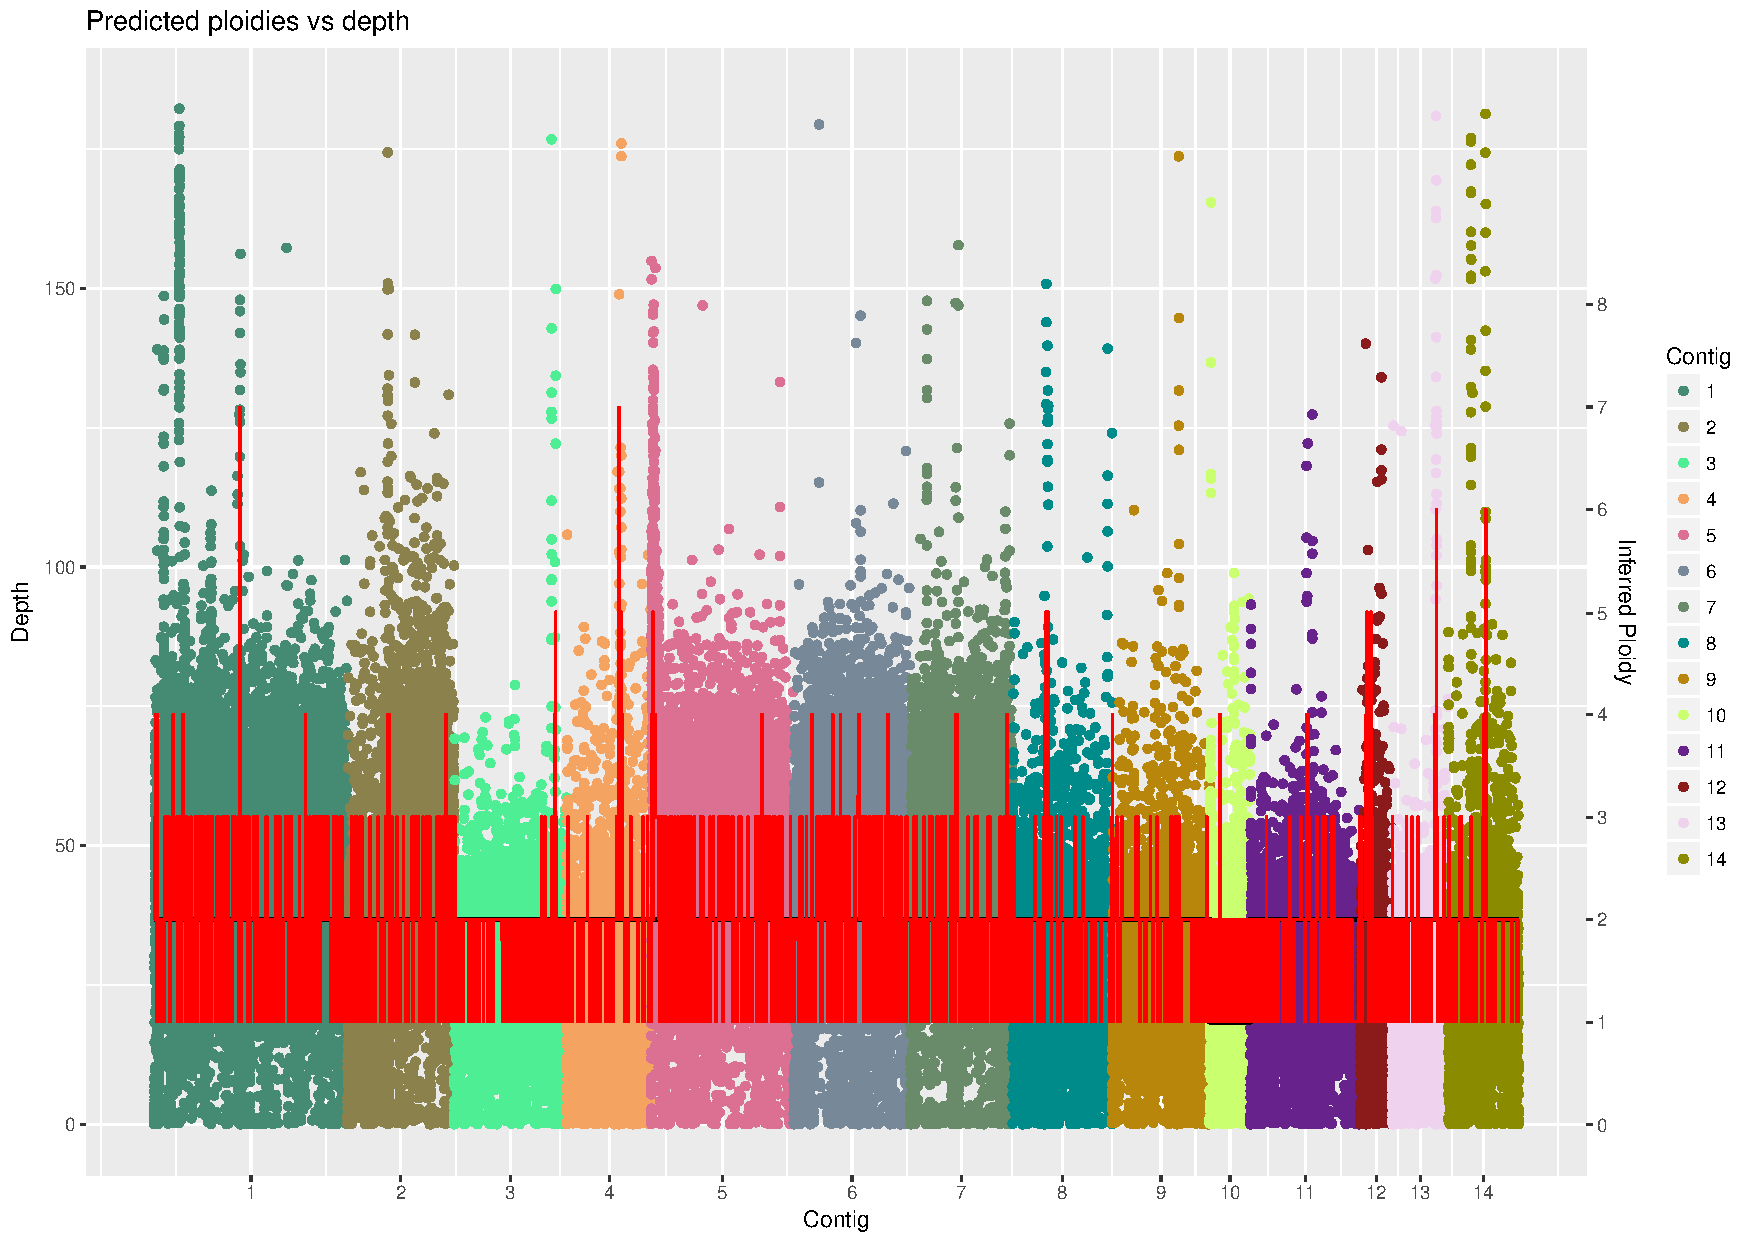
\includegraphics[scale=0.5]{Plots/Sample_7_plot.pdf}
\end{center}
\end{figure}
\begin{figure}[H]
\begin{center}
\caption{CCTP50-d257}
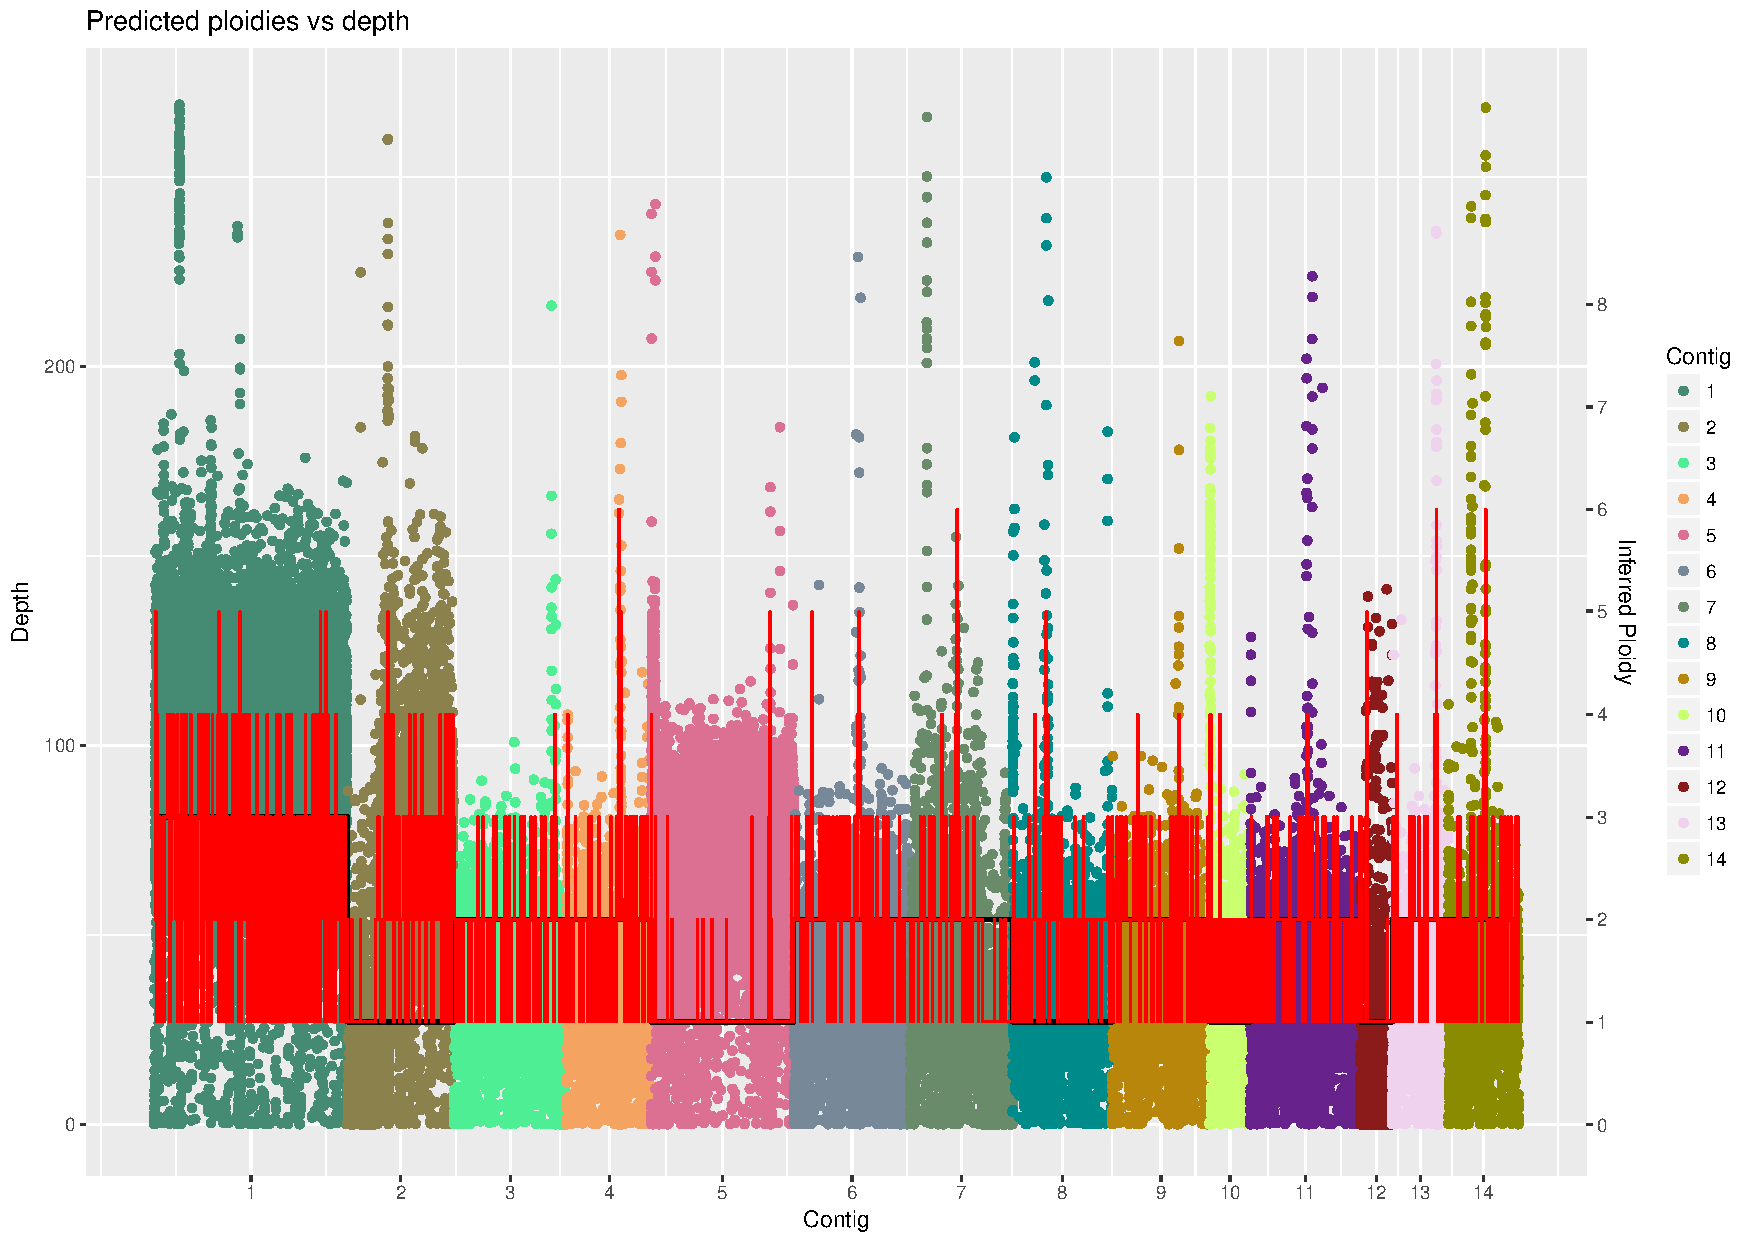
\includegraphics[scale=0.5]{Plots/Sample_5_plot.pdf}
\end{center}
\end{figure}
\begin{figure}[H]
\begin{center}
\caption{IFNR23}
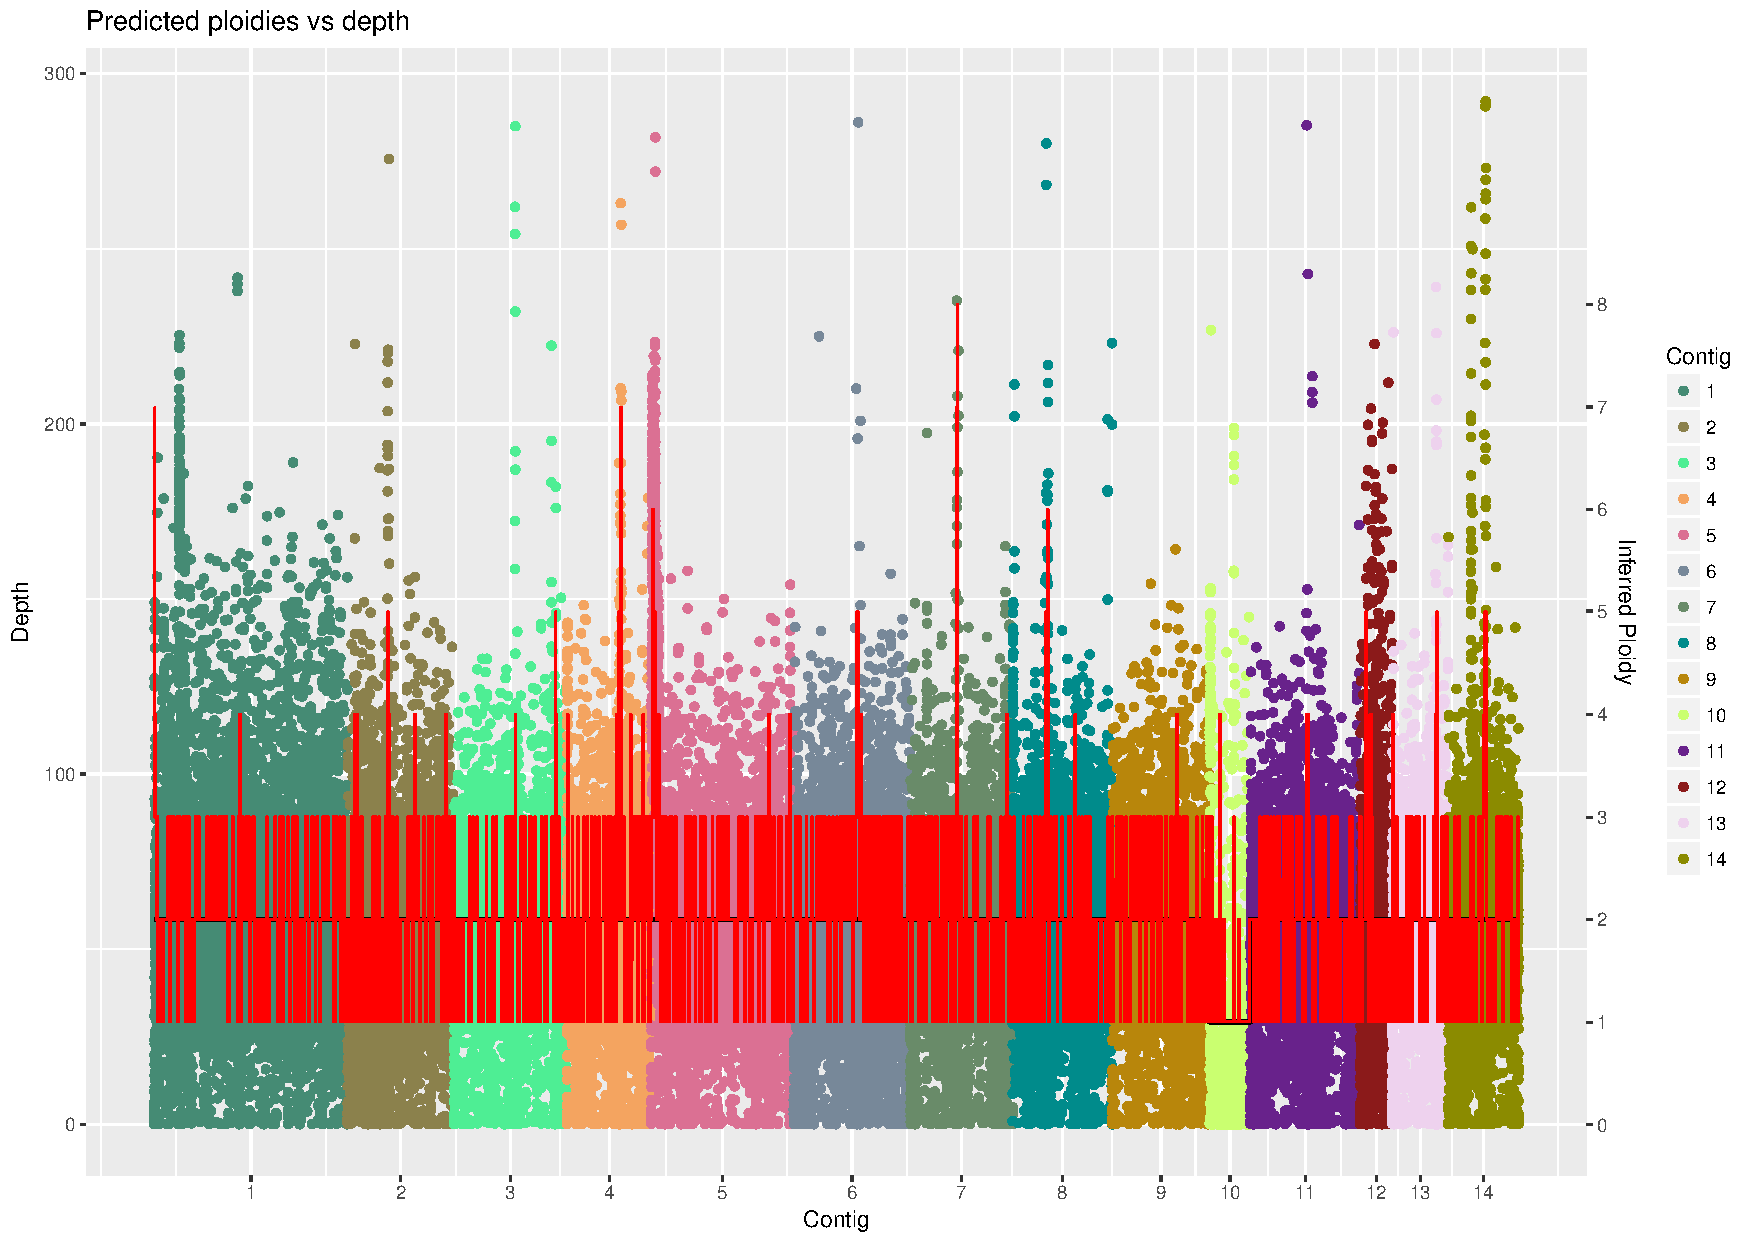
\includegraphics[scale=0.5]{Plots/Sample_16_plot.pdf}
\end{center}
\end{figure}
\begin{figure}[H]
\begin{center}
\caption{IFNR23-d179}
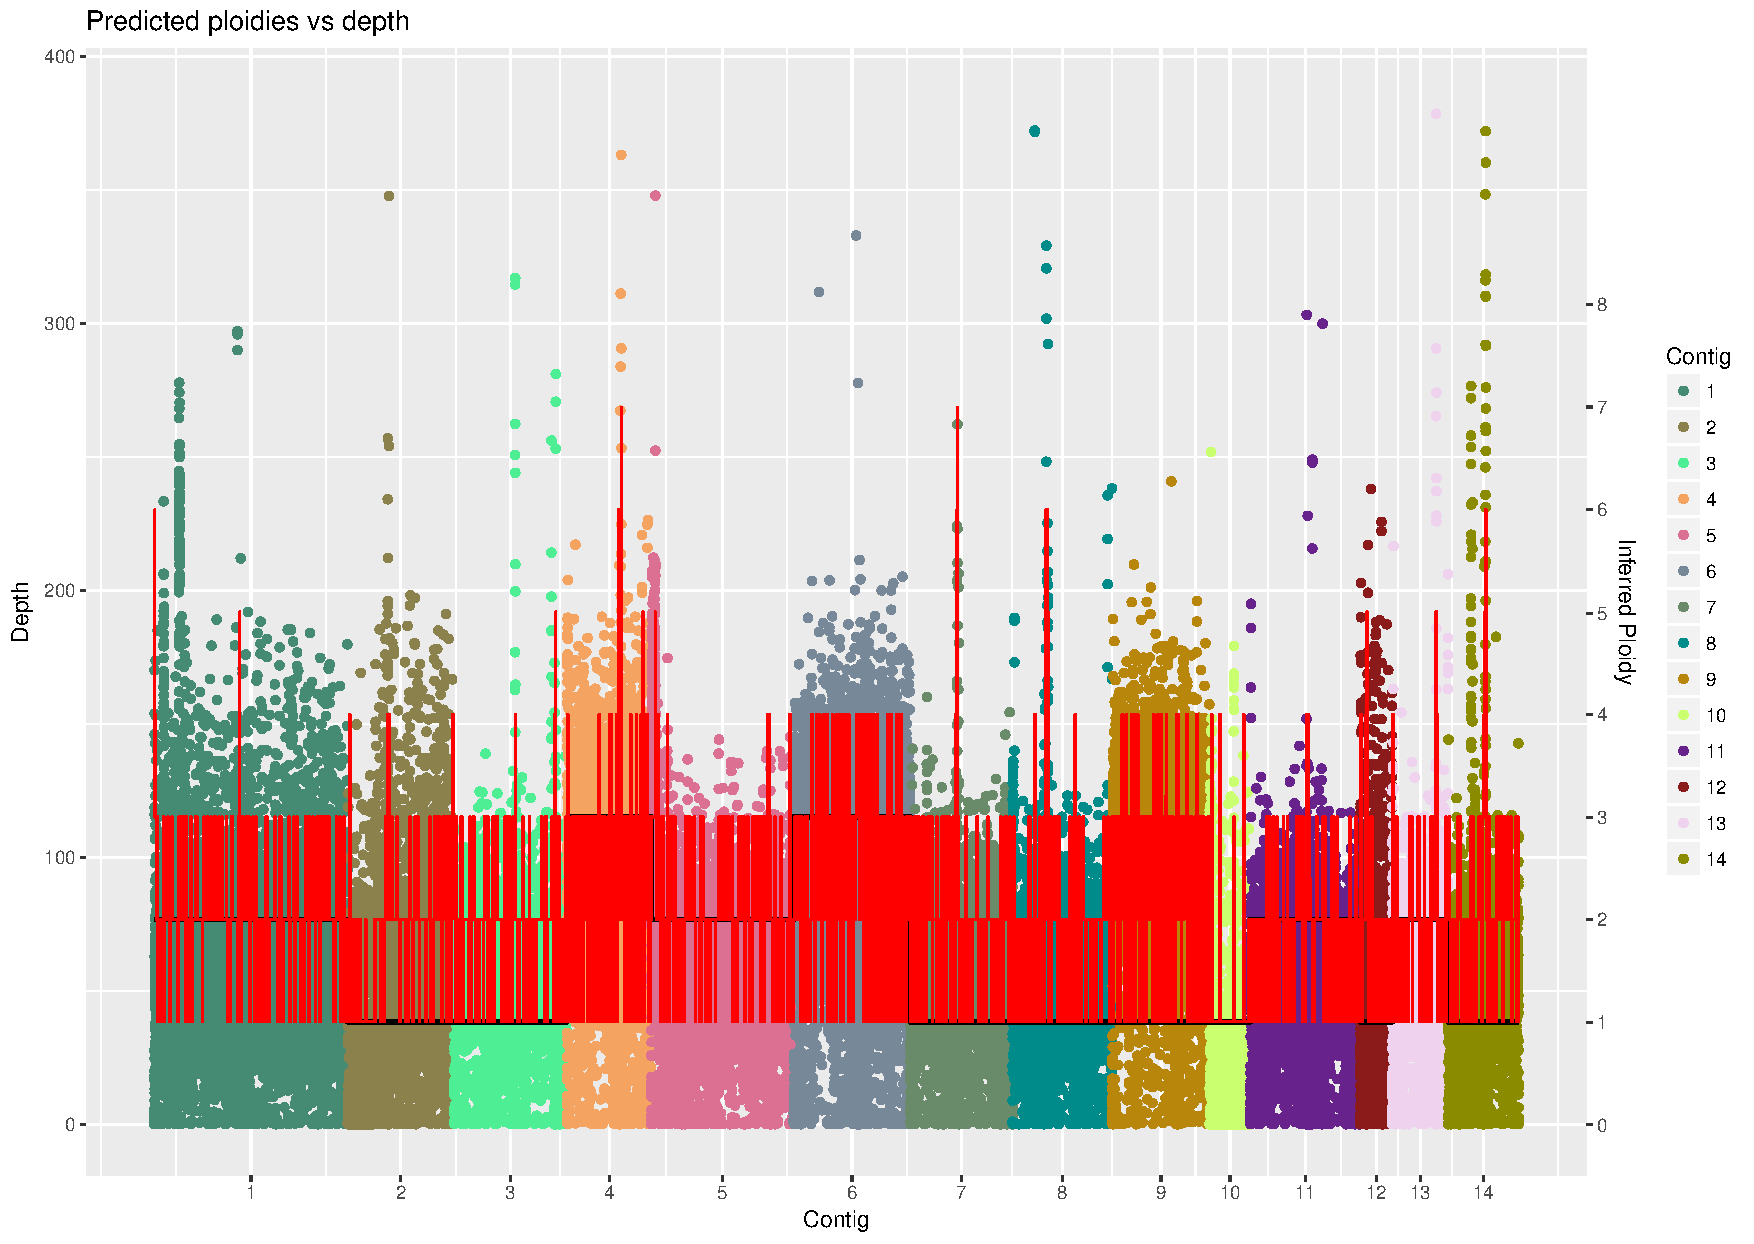
\includegraphics[scale=0.5]{Plots/Sample_15_plot.pdf}
\end{center}
\end{figure}
When all other samples were run, the only other occurrence of aneuploidy was found in the sample CCTP50-d409.
\begin{figure}[H]
\begin{center}
\caption{CCTP-d409}
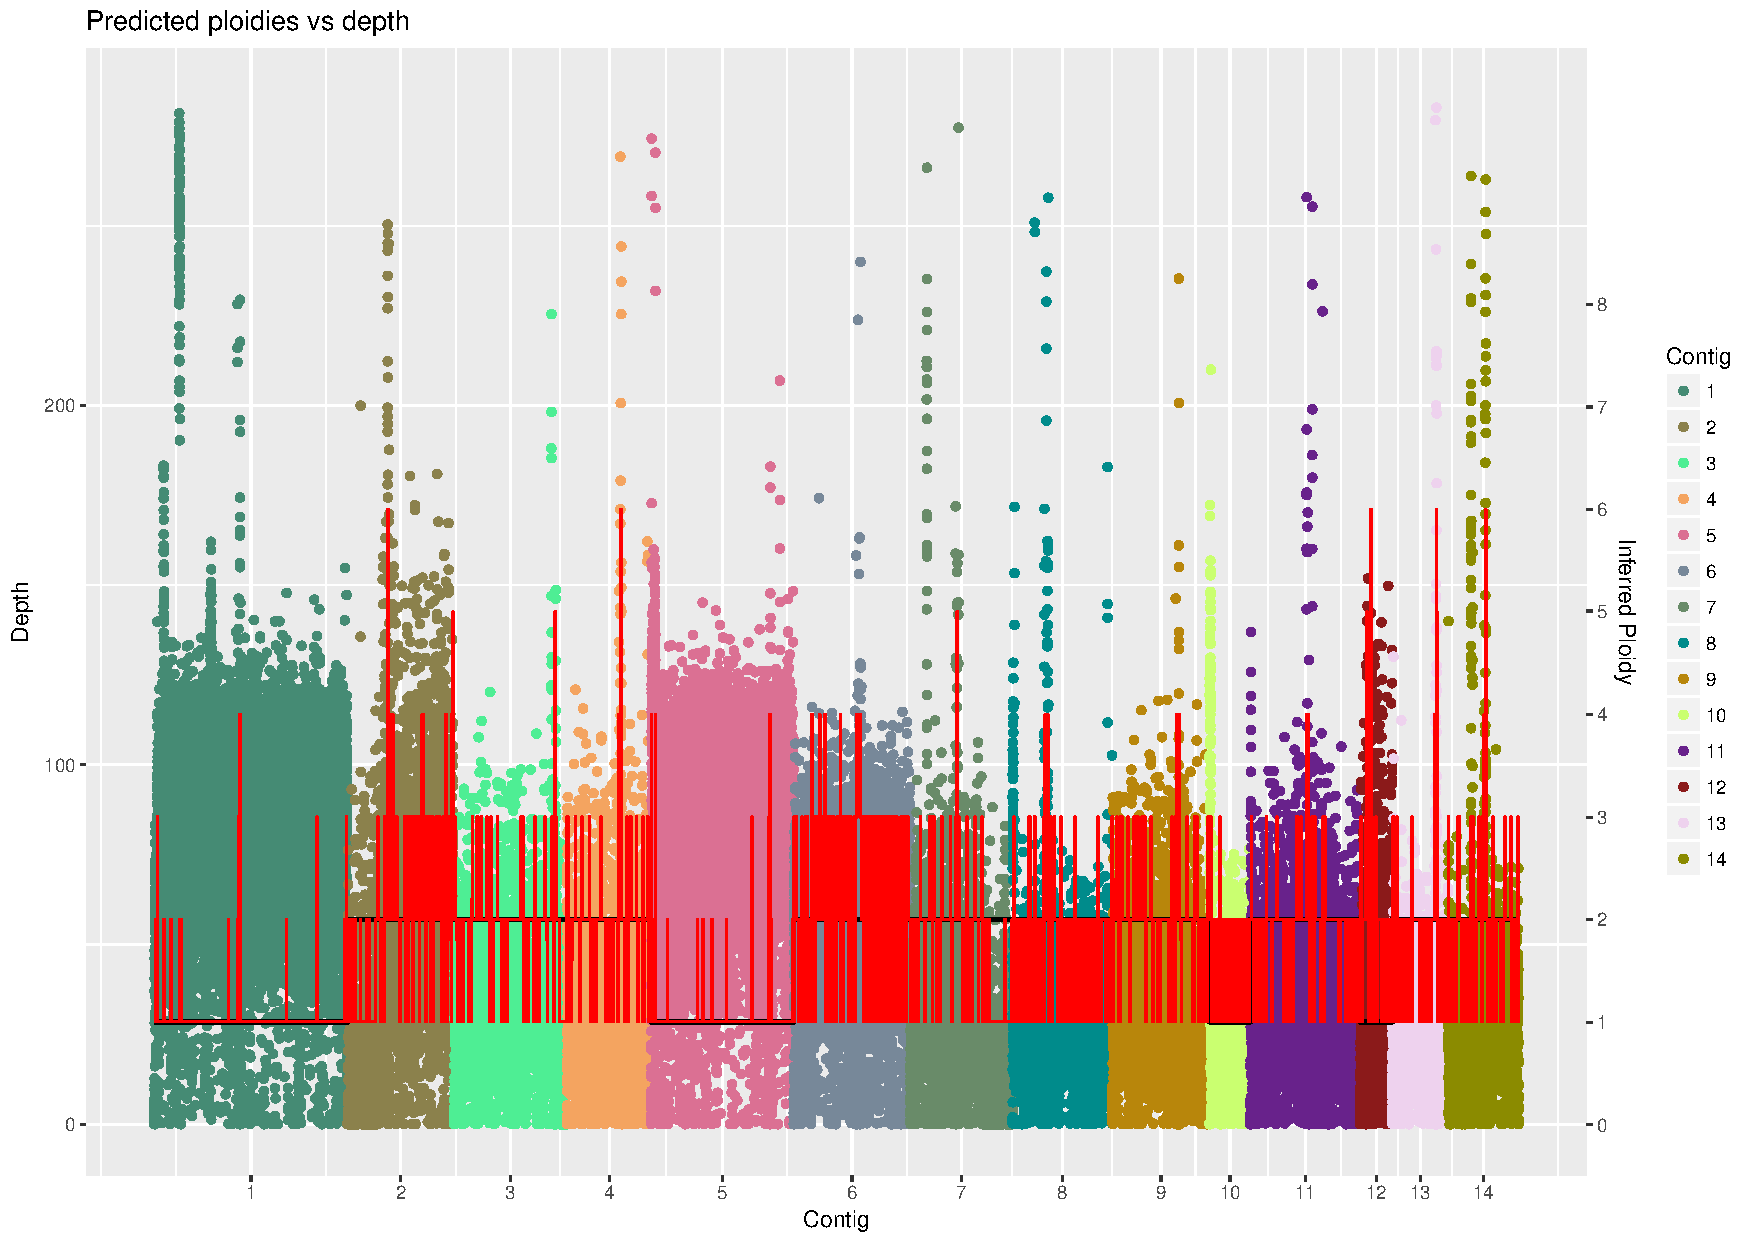
\includegraphics[scale=0.5]{Plots/Sample_6_plot.pdf}
\end{center}
\end{figure}
All other samples came out as being haploid across the entire genome. The samples with aneuploidy are all from the VNB lineage which has been identified as being the most lineage with the greatest level of aneuploidy \autocite{Rhodes2017}. The paper also identified the IFNR23 sample as a hypermuator which explains the large quantity of aneuploidy detected in IFNR23 and its post treatment isolate IFNR23-d179.   
\section{Discussion}
\section{Conclusion}
\section{Acknowledgements}

\pagebreak 
\printbibliography
\pagebreak
\end{document}